\documentclass[twoside]{book}

% Packages required by doxygen
\usepackage{fixltx2e}
\usepackage{calc}
\usepackage{doxygen}
\usepackage[export]{adjustbox} % also loads graphicx
\usepackage{graphicx}
\usepackage[utf8]{inputenc}
\usepackage{makeidx}
\usepackage{multicol}
\usepackage{multirow}
\PassOptionsToPackage{warn}{textcomp}
\usepackage{textcomp}
\usepackage[nointegrals]{wasysym}
\usepackage[table]{xcolor}

% Font selection
\usepackage[T1]{fontenc}
\usepackage[scaled=.90]{helvet}
\usepackage{courier}
\usepackage{amssymb}
\usepackage{sectsty}
\renewcommand{\familydefault}{\sfdefault}
\allsectionsfont{%
  \fontseries{bc}\selectfont%
  \color{darkgray}%
}
\renewcommand{\DoxyLabelFont}{%
  \fontseries{bc}\selectfont%
  \color{darkgray}%
}
\newcommand{\+}{\discretionary{\mbox{\scriptsize$\hookleftarrow$}}{}{}}

% Page & text layout
\usepackage{geometry}
\geometry{%
  a4paper,%
  top=2.5cm,%
  bottom=2.5cm,%
  left=2.5cm,%
  right=2.5cm%
}
\tolerance=750
\hfuzz=15pt
\hbadness=750
\setlength{\emergencystretch}{15pt}
\setlength{\parindent}{0cm}
\setlength{\parskip}{3ex plus 2ex minus 2ex}
\makeatletter
\renewcommand{\paragraph}{%
  \@startsection{paragraph}{4}{0ex}{-1.0ex}{1.0ex}{%
    \normalfont\normalsize\bfseries\SS@parafont%
  }%
}
\renewcommand{\subparagraph}{%
  \@startsection{subparagraph}{5}{0ex}{-1.0ex}{1.0ex}{%
    \normalfont\normalsize\bfseries\SS@subparafont%
  }%
}
\makeatother

% Headers & footers
\usepackage{fancyhdr}
\pagestyle{fancyplain}
\fancyhead[LE]{\fancyplain{}{\bfseries\thepage}}
\fancyhead[CE]{\fancyplain{}{}}
\fancyhead[RE]{\fancyplain{}{\bfseries\leftmark}}
\fancyhead[LO]{\fancyplain{}{\bfseries\rightmark}}
\fancyhead[CO]{\fancyplain{}{}}
\fancyhead[RO]{\fancyplain{}{\bfseries\thepage}}
\fancyfoot[LE]{\fancyplain{}{}}
\fancyfoot[CE]{\fancyplain{}{}}
\fancyfoot[RE]{\fancyplain{}{\bfseries\scriptsize Generated by Doxygen }}
\fancyfoot[LO]{\fancyplain{}{\bfseries\scriptsize Generated by Doxygen }}
\fancyfoot[CO]{\fancyplain{}{}}
\fancyfoot[RO]{\fancyplain{}{}}
\renewcommand{\footrulewidth}{0.4pt}
\renewcommand{\chaptermark}[1]{%
  \markboth{#1}{}%
}
\renewcommand{\sectionmark}[1]{%
  \markright{\thesection\ #1}%
}

% Indices & bibliography
\usepackage{natbib}
\usepackage[titles]{tocloft}
\setcounter{tocdepth}{3}
\setcounter{secnumdepth}{5}
\makeindex

% Hyperlinks (required, but should be loaded last)
\usepackage{ifpdf}
\ifpdf
  \usepackage[pdftex,pagebackref=true]{hyperref}
\else
  \usepackage[ps2pdf,pagebackref=true]{hyperref}
\fi
\hypersetup{%
  colorlinks=true,%
  linkcolor=blue,%
  citecolor=blue,%
  unicode%
}

% Custom commands
\newcommand{\clearemptydoublepage}{%
  \newpage{\pagestyle{empty}\cleardoublepage}%
}

\usepackage{caption}
\captionsetup{labelsep=space,justification=centering,font={bf},singlelinecheck=off,skip=4pt,position=top}

%===== C O N T E N T S =====

\begin{document}

% Titlepage & ToC
\hypersetup{pageanchor=false,
             bookmarksnumbered=true,
             pdfencoding=unicode
            }
\pagenumbering{alph}
\begin{titlepage}
\vspace*{7cm}
\begin{center}%
{\Large shell }\\
\vspace*{1cm}
{\large Generated by Doxygen 1.8.13}\\
\end{center}
\end{titlepage}
\clearemptydoublepage
\pagenumbering{roman}
\tableofcontents
\clearemptydoublepage
\pagenumbering{arabic}
\hypersetup{pageanchor=true}

%--- Begin generated contents ---
\chapter{shell -\/ Description.}
\label{index}\hypertarget{index}{} 
\chapter{File Index}
\section{File List}
Here is a list of all documented files with brief descriptions\+:\begin{DoxyCompactList}
\item\contentsline{section}{\hyperlink{commands_8c}{commands.\+c} }{\pageref{commands_8c}}{}
\item\contentsline{section}{\hyperlink{executor_8c}{executor.\+c} }{\pageref{executor_8c}}{}
\item\contentsline{section}{\hyperlink{history_8c}{history.\+c} }{\pageref{history_8c}}{}
\item\contentsline{section}{\hyperlink{reader_8c}{reader.\+c} }{\pageref{reader_8c}}{}
\item\contentsline{section}{\hyperlink{shell_8c}{shell.\+c} }{\pageref{shell_8c}}{}
\item\contentsline{section}{\hyperlink{shell_8h}{shell.\+h} }{\pageref{shell_8h}}{}
\item\contentsline{section}{\hyperlink{signals_8c}{signals.\+c} }{\pageref{signals_8c}}{}
\item\contentsline{section}{\hyperlink{time_8c}{time.\+c} }{\pageref{time_8c}}{}
\end{DoxyCompactList}

\chapter{File Documentation}
\hypertarget{commands_8c}{}\section{commands.\+c File Reference}
\label{commands_8c}\index{commands.\+c@{commands.\+c}}
{\ttfamily \#include \char`\"{}shell.\+h\char`\"{}}\newline
\subsection*{Functions}
\begin{DoxyCompactItemize}
\item 
int \hyperlink{commands_8c_a069f9558baae3a064ba0e1b54456ccab}{cd} (char $\ast$$\ast$args)
\begin{DoxyCompactList}\small\item\em Change directory command. \end{DoxyCompactList}\item 
int \hyperlink{commands_8c_a3224f605963ffa2708e3e4cc3d8bb41e}{execute\+\_\+command} (int command\+\_\+number, char $\ast$$\ast$args)
\begin{DoxyCompactList}\small\item\em Calls built-\/in command. \end{DoxyCompactList}\item 
int \hyperlink{commands_8c_a13166be76043b3dfccc0f830c846dc26}{help} ()
\begin{DoxyCompactList}\small\item\em Prints list of built-\/in commands and other functionalities. \end{DoxyCompactList}\item 
int \hyperlink{commands_8c_a480f710944fe509e060ee055ff64fa88}{print\+\_\+time} ()
\begin{DoxyCompactList}\small\item\em Prints current date and time. \end{DoxyCompactList}\end{DoxyCompactItemize}


\subsection{Detailed Description}
\begin{DoxyAuthor}{Author}
Mateusz Wawreszuk 
\end{DoxyAuthor}


\subsection{Function Documentation}
\mbox{\Hypertarget{commands_8c_a069f9558baae3a064ba0e1b54456ccab}\label{commands_8c_a069f9558baae3a064ba0e1b54456ccab}} 
\index{commands.\+c@{commands.\+c}!cd@{cd}}
\index{cd@{cd}!commands.\+c@{commands.\+c}}
\subsubsection{\texorpdfstring{cd()}{cd()}}
{\footnotesize\ttfamily int cd (\begin{DoxyParamCaption}\item[{char $\ast$$\ast$}]{args }\end{DoxyParamCaption})}



Change directory command. 

If change is not possible, prints to standard output error message.


\begin{DoxyParams}{Parameters}
{\em args} & directory \\
\hline
\end{DoxyParams}
\begin{DoxyReturn}{Returns}
execution success or error code 
\end{DoxyReturn}
\mbox{\Hypertarget{commands_8c_a3224f605963ffa2708e3e4cc3d8bb41e}\label{commands_8c_a3224f605963ffa2708e3e4cc3d8bb41e}} 
\index{commands.\+c@{commands.\+c}!execute\+\_\+command@{execute\+\_\+command}}
\index{execute\+\_\+command@{execute\+\_\+command}!commands.\+c@{commands.\+c}}
\subsubsection{\texorpdfstring{execute\+\_\+command()}{execute\_command()}}
{\footnotesize\ttfamily int execute\+\_\+command (\begin{DoxyParamCaption}\item[{int}]{command\+\_\+number,  }\item[{char $\ast$$\ast$}]{args }\end{DoxyParamCaption})}



Calls built-\/in command. 


\begin{DoxyParams}{Parameters}
{\em command\+\_\+number} & number of command in built\+\_\+in\+\_\+commands array \\
\hline
{\em args} & arguments \\
\hline
\end{DoxyParams}
\begin{DoxyReturn}{Returns}
execution success or error code 
\end{DoxyReturn}
\mbox{\Hypertarget{commands_8c_a13166be76043b3dfccc0f830c846dc26}\label{commands_8c_a13166be76043b3dfccc0f830c846dc26}} 
\index{commands.\+c@{commands.\+c}!help@{help}}
\index{help@{help}!commands.\+c@{commands.\+c}}
\subsubsection{\texorpdfstring{help()}{help()}}
{\footnotesize\ttfamily int help (\begin{DoxyParamCaption}{ }\end{DoxyParamCaption})}



Prints list of built-\/in commands and other functionalities. 

\begin{DoxyReturn}{Returns}
success code 
\end{DoxyReturn}
\mbox{\Hypertarget{commands_8c_a480f710944fe509e060ee055ff64fa88}\label{commands_8c_a480f710944fe509e060ee055ff64fa88}} 
\index{commands.\+c@{commands.\+c}!print\+\_\+time@{print\+\_\+time}}
\index{print\+\_\+time@{print\+\_\+time}!commands.\+c@{commands.\+c}}
\subsubsection{\texorpdfstring{print\+\_\+time()}{print\_time()}}
{\footnotesize\ttfamily int print\+\_\+time (\begin{DoxyParamCaption}{ }\end{DoxyParamCaption})}



Prints current date and time. 

\begin{DoxyReturn}{Returns}
success code 
\end{DoxyReturn}

\hypertarget{executor_8c}{}\section{executor.\+c File Reference}
\label{executor_8c}\index{executor.\+c@{executor.\+c}}
{\ttfamily \#include \char`\"{}shell.\+h\char`\"{}}\newline
\subsection*{Functions}
\begin{DoxyCompactItemize}
\item 
int \hyperlink{executor_8c_a38ce9fb8be12b03640a8f1c94a8e4f2c}{execute\+\_\+command\+\_\+or\+\_\+program} (char $\ast$$\ast$args)
\begin{DoxyCompactList}\small\item\em Calls built-\/in command or executes external program. \end{DoxyCompactList}\item 
int \hyperlink{executor_8c_a686fef0ad33bc5f90fcabc31276090f5}{execute\+\_\+program} (char $\ast$$\ast$args, int exec\+\_\+in\+\_\+bg)
\begin{DoxyCompactList}\small\item\em Executes external program. \end{DoxyCompactList}\item 
void \hyperlink{executor_8c_a5b063ff4b62fde90e1a44e8c89d5ebc6}{print\+\_\+process\+\_\+signal} (int signum)
\begin{DoxyCompactList}\small\item\em Prints information witch process has been killed. \end{DoxyCompactList}\end{DoxyCompactItemize}
\subsection*{Variables}
\begin{DoxyCompactItemize}
\item 
\mbox{\Hypertarget{executor_8c_a763303be5a9ead1e6065ffc2340b01fc}\label{executor_8c_a763303be5a9ead1e6065ffc2340b01fc}} 
char $\ast$ \hyperlink{executor_8c_a763303be5a9ead1e6065ffc2340b01fc}{built\+\_\+in\+\_\+commands} \mbox{[}$\,$\mbox{]} = \{\char`\"{}cd\char`\"{}, \char`\"{}\hyperlink{shell_8h_a13166be76043b3dfccc0f830c846dc26}{help}\char`\"{}, \char`\"{}history\char`\"{}, \char`\"{}time\char`\"{}, \char`\"{}exit\char`\"{}\}
\begin{DoxyCompactList}\small\item\em Array of built in commands. \end{DoxyCompactList}\item 
\mbox{\Hypertarget{executor_8c_a7c855d8edb504957177d3eb3904cd9be}\label{executor_8c_a7c855d8edb504957177d3eb3904cd9be}} 
char \hyperlink{executor_8c_a7c855d8edb504957177d3eb3904cd9be}{active\+\_\+process\+\_\+name} \mbox{[}\hyperlink{shell_8h_aa9b8dcc02cea15aab8e3d0b7860327a7}{I\+N\+P\+U\+T\+\_\+\+B\+U\+F\+F\+E\+R\+\_\+\+S\+I\+ZE}\mbox{]}
\begin{DoxyCompactList}\small\item\em Last executed program name. \end{DoxyCompactList}\item 
\mbox{\Hypertarget{executor_8c_a1239c1ad5d45564a81c1e3b8e01aeb98}\label{executor_8c_a1239c1ad5d45564a81c1e3b8e01aeb98}} 
int \hyperlink{executor_8c_a1239c1ad5d45564a81c1e3b8e01aeb98}{active\+\_\+process\+\_\+id}
\begin{DoxyCompactList}\small\item\em Id of process that executes program. \end{DoxyCompactList}\end{DoxyCompactItemize}


\subsection{Detailed Description}
\begin{DoxyAuthor}{Author}
Mateusz Wawreszuk 
\end{DoxyAuthor}


\subsection{Function Documentation}
\mbox{\Hypertarget{executor_8c_a38ce9fb8be12b03640a8f1c94a8e4f2c}\label{executor_8c_a38ce9fb8be12b03640a8f1c94a8e4f2c}} 
\index{executor.\+c@{executor.\+c}!execute\+\_\+command\+\_\+or\+\_\+program@{execute\+\_\+command\+\_\+or\+\_\+program}}
\index{execute\+\_\+command\+\_\+or\+\_\+program@{execute\+\_\+command\+\_\+or\+\_\+program}!executor.\+c@{executor.\+c}}
\subsubsection{\texorpdfstring{execute\+\_\+command\+\_\+or\+\_\+program()}{execute\_command\_or\_program()}}
{\footnotesize\ttfamily int execute\+\_\+command\+\_\+or\+\_\+program (\begin{DoxyParamCaption}\item[{char $\ast$$\ast$}]{args }\end{DoxyParamCaption})}



Calls built-\/in command or executes external program. 

Checks if program should be executed in background (first argument is \char`\"{}\&\char`\"{}).


\begin{DoxyParams}{Parameters}
{\em args} & array of command and its arguments \\
\hline
\end{DoxyParams}
\begin{DoxyReturn}{Returns}
execution success or error code 
\end{DoxyReturn}
\mbox{\Hypertarget{executor_8c_a686fef0ad33bc5f90fcabc31276090f5}\label{executor_8c_a686fef0ad33bc5f90fcabc31276090f5}} 
\index{executor.\+c@{executor.\+c}!execute\+\_\+program@{execute\+\_\+program}}
\index{execute\+\_\+program@{execute\+\_\+program}!executor.\+c@{executor.\+c}}
\subsubsection{\texorpdfstring{execute\+\_\+program()}{execute\_program()}}
{\footnotesize\ttfamily int execute\+\_\+program (\begin{DoxyParamCaption}\item[{char $\ast$$\ast$}]{args,  }\item[{int}]{exec\+\_\+in\+\_\+bg }\end{DoxyParamCaption})}



Executes external program. 


\begin{DoxyParams}{Parameters}
{\em args} & array of command and its arguments \\
\hline
{\em exec\+\_\+in\+\_\+bg} & 1 if program should be executed in background, 0 if not \\
\hline
\end{DoxyParams}
\begin{DoxyReturn}{Returns}
W\+Y\+J\+S\+C\+IE 
\end{DoxyReturn}
\mbox{\Hypertarget{executor_8c_a5b063ff4b62fde90e1a44e8c89d5ebc6}\label{executor_8c_a5b063ff4b62fde90e1a44e8c89d5ebc6}} 
\index{executor.\+c@{executor.\+c}!print\+\_\+process\+\_\+signal@{print\+\_\+process\+\_\+signal}}
\index{print\+\_\+process\+\_\+signal@{print\+\_\+process\+\_\+signal}!executor.\+c@{executor.\+c}}
\subsubsection{\texorpdfstring{print\+\_\+process\+\_\+signal()}{print\_process\_signal()}}
{\footnotesize\ttfamily void print\+\_\+process\+\_\+signal (\begin{DoxyParamCaption}\item[{int}]{signum }\end{DoxyParamCaption})}



Prints information witch process has been killed. 


\begin{DoxyParams}{Parameters}
{\em signum} & signal number \\
\hline
\end{DoxyParams}

\hypertarget{history_8c}{}\section{history.\+c File Reference}
\label{history_8c}\index{history.\+c@{history.\+c}}
{\ttfamily \#include \char`\"{}shell.\+h\char`\"{}}\newline
\subsection*{Functions}
\begin{DoxyCompactItemize}
\item 
\mbox{\Hypertarget{history_8c_a5fb80f885af4c12056db03cc45a6aae9}\label{history_8c_a5fb80f885af4c12056db03cc45a6aae9}} 
void \hyperlink{history_8c_a5fb80f885af4c12056db03cc45a6aae9}{history\+\_\+clean\+\_\+up} ()
\begin{DoxyCompactList}\small\item\em Frees memory, saves commands history to file. \end{DoxyCompactList}\item 
void \hyperlink{history_8c_ae8516142b2cb36ede692dfca4a36d8cc}{initialize\+\_\+commands\+\_\+history} ()
\begin{DoxyCompactList}\small\item\em Initializes commands history. \end{DoxyCompactList}\item 
int \hyperlink{history_8c_abcf676d5284d55cb7835a81a80619a48}{print\+\_\+history} ()
\begin{DoxyCompactList}\small\item\em Prints commands history to standard output. \end{DoxyCompactList}\item 
\mbox{\Hypertarget{history_8c_ac4ba99969792ae3f877c857cedb129a9}\label{history_8c_ac4ba99969792ae3f877c857cedb129a9}} 
void \hyperlink{history_8c_ac4ba99969792ae3f877c857cedb129a9}{save\+\_\+history\+\_\+to\+\_\+file} ()
\begin{DoxyCompactList}\small\item\em Saves command\+\_\+history array to file. \end{DoxyCompactList}\item 
void \hyperlink{history_8c_aca67f770a00272dc2993db7d854c9c48}{save\+\_\+to\+\_\+history} (char $\ast$input)
\begin{DoxyCompactList}\small\item\em Saves command to history. \end{DoxyCompactList}\end{DoxyCompactItemize}
\subsection*{Variables}
\begin{DoxyCompactItemize}
\item 
\mbox{\Hypertarget{history_8c_a52ed4b61ce335f0c68e3fb90487fe512}\label{history_8c_a52ed4b61ce335f0c68e3fb90487fe512}} 
char $\ast$$\ast$ \hyperlink{history_8c_a52ed4b61ce335f0c68e3fb90487fe512}{commands\+\_\+history}
\begin{DoxyCompactList}\small\item\em Array to store commands history. \end{DoxyCompactList}\item 
\mbox{\Hypertarget{history_8c_a259d6d81496e72255f0b1222ed592dde}\label{history_8c_a259d6d81496e72255f0b1222ed592dde}} 
char $\ast$ \hyperlink{history_8c_a259d6d81496e72255f0b1222ed592dde}{history\+\_\+file\+\_\+path}
\begin{DoxyCompactList}\small\item\em Commands history file path -\/ users home directory. \end{DoxyCompactList}\item 
\mbox{\Hypertarget{history_8c_a73081c43fc7a8aac4707723496bb02dc}\label{history_8c_a73081c43fc7a8aac4707723496bb02dc}} 
volatile int \hyperlink{history_8c_a73081c43fc7a8aac4707723496bb02dc}{history\+\_\+counter} = 0
\begin{DoxyCompactList}\small\item\em Pointer to last position in commands history array. \end{DoxyCompactList}\end{DoxyCompactItemize}


\subsection{Detailed Description}
\begin{DoxyAuthor}{Author}
Mateusz Wawreszuk 
\end{DoxyAuthor}


\subsection{Function Documentation}
\mbox{\Hypertarget{history_8c_ae8516142b2cb36ede692dfca4a36d8cc}\label{history_8c_ae8516142b2cb36ede692dfca4a36d8cc}} 
\index{history.\+c@{history.\+c}!initialize\+\_\+commands\+\_\+history@{initialize\+\_\+commands\+\_\+history}}
\index{initialize\+\_\+commands\+\_\+history@{initialize\+\_\+commands\+\_\+history}!history.\+c@{history.\+c}}
\subsubsection{\texorpdfstring{initialize\+\_\+commands\+\_\+history()}{initialize\_commands\_history()}}
{\footnotesize\ttfamily void initialize\+\_\+commands\+\_\+history (\begin{DoxyParamCaption}{ }\end{DoxyParamCaption})}



Initializes commands history. 

Allocates commands\+\_\+history array and reads current history from file. Sets history\+\_\+counter pointer to commands\+\_\+history size. \mbox{\Hypertarget{history_8c_abcf676d5284d55cb7835a81a80619a48}\label{history_8c_abcf676d5284d55cb7835a81a80619a48}} 
\index{history.\+c@{history.\+c}!print\+\_\+history@{print\+\_\+history}}
\index{print\+\_\+history@{print\+\_\+history}!history.\+c@{history.\+c}}
\subsubsection{\texorpdfstring{print\+\_\+history()}{print\_history()}}
{\footnotesize\ttfamily int print\+\_\+history (\begin{DoxyParamCaption}{ }\end{DoxyParamCaption})}



Prints commands history to standard output. 

\begin{DoxyReturn}{Returns}
success code 
\end{DoxyReturn}
\mbox{\Hypertarget{history_8c_aca67f770a00272dc2993db7d854c9c48}\label{history_8c_aca67f770a00272dc2993db7d854c9c48}} 
\index{history.\+c@{history.\+c}!save\+\_\+to\+\_\+history@{save\+\_\+to\+\_\+history}}
\index{save\+\_\+to\+\_\+history@{save\+\_\+to\+\_\+history}!history.\+c@{history.\+c}}
\subsubsection{\texorpdfstring{save\+\_\+to\+\_\+history()}{save\_to\_history()}}
{\footnotesize\ttfamily void save\+\_\+to\+\_\+history (\begin{DoxyParamCaption}\item[{char $\ast$}]{input }\end{DoxyParamCaption})}



Saves command to history. 

If history\+\_\+counter pointer points that history is full, removes first command from history.


\begin{DoxyParams}{Parameters}
{\em input} & command to save \\
\hline
\end{DoxyParams}

\hypertarget{reader_8c}{}\section{reader.\+c File Reference}
\label{reader_8c}\index{reader.\+c@{reader.\+c}}
{\ttfamily \#include \char`\"{}shell.\+h\char`\"{}}\newline
\subsection*{Functions}
\begin{DoxyCompactItemize}
\item 
\mbox{\Hypertarget{reader_8c_aa2deaf0f63ca4a73a37b86d05678fb46}\label{reader_8c_aa2deaf0f63ca4a73a37b86d05678fb46}} 
void \hyperlink{reader_8c_aa2deaf0f63ca4a73a37b86d05678fb46}{main\+\_\+loop} ()
\begin{DoxyCompactList}\small\item\em Waits for input and executes it. \end{DoxyCompactList}\item 
void \hyperlink{reader_8c_a87a73ece208da0ed13ff48923efa6a8f}{main\+\_\+loop\+\_\+file} (char $\ast$filename)
\begin{DoxyCompactList}\small\item\em Reads script file and executes every line. \end{DoxyCompactList}\item 
void \hyperlink{reader_8c_a21579a20737c3b2b24e18bb5e51d8140}{print\+\_\+prompt} ()
\begin{DoxyCompactList}\small\item\em Prints command prompt. \end{DoxyCompactList}\item 
\mbox{\Hypertarget{reader_8c_a6d4d28fe8b4a7cad21ec581450abe1b1}\label{reader_8c_a6d4d28fe8b4a7cad21ec581450abe1b1}} 
void \hyperlink{reader_8c_a6d4d28fe8b4a7cad21ec581450abe1b1}{read\+\_\+clean\+\_\+up} ()
\begin{DoxyCompactList}\small\item\em Frees memory. \end{DoxyCompactList}\item 
char $\ast$ \hyperlink{reader_8c_a777131faf4806e7eee788b65cab4a584}{read\+\_\+line} ()
\begin{DoxyCompactList}\small\item\em Reads one line from standard input. \end{DoxyCompactList}\item 
char $\ast$$\ast$ \hyperlink{reader_8c_a9c985d892b630e70b2236554b46faa4b}{split\+\_\+input} (char $\ast$input)
\begin{DoxyCompactList}\small\item\em Splits input to words (command and its arguments). \end{DoxyCompactList}\item 
\mbox{\Hypertarget{reader_8c_a62b3e552188dc2021715c1be2bd60267}\label{reader_8c_a62b3e552188dc2021715c1be2bd60267}} 
void \hyperlink{reader_8c_a62b3e552188dc2021715c1be2bd60267}{update\+\_\+prompt} ()
\begin{DoxyCompactList}\small\item\em Updates prompt with username and current path. \end{DoxyCompactList}\end{DoxyCompactItemize}
\subsection*{Variables}
\begin{DoxyCompactItemize}
\item 
\mbox{\Hypertarget{reader_8c_a5332aadd744ac89bd68c49c14286adeb}\label{reader_8c_a5332aadd744ac89bd68c49c14286adeb}} 
char $\ast$ \hyperlink{reader_8c_a5332aadd744ac89bd68c49c14286adeb}{command\+\_\+prompt}
\begin{DoxyCompactList}\small\item\em Array of characters to store command prompt. \end{DoxyCompactList}\item 
\mbox{\Hypertarget{reader_8c_a9b20c006bd90a09e1465fb668700e81d}\label{reader_8c_a9b20c006bd90a09e1465fb668700e81d}} 
char $\ast$ \hyperlink{reader_8c_a9b20c006bd90a09e1465fb668700e81d}{username}
\begin{DoxyCompactList}\small\item\em Array of characters to store current users name. \end{DoxyCompactList}\end{DoxyCompactItemize}


\subsection{Detailed Description}
\begin{DoxyAuthor}{Author}
Mateusz Wawreszuk 
\end{DoxyAuthor}


\subsection{Function Documentation}
\mbox{\Hypertarget{reader_8c_a87a73ece208da0ed13ff48923efa6a8f}\label{reader_8c_a87a73ece208da0ed13ff48923efa6a8f}} 
\index{reader.\+c@{reader.\+c}!main\+\_\+loop\+\_\+file@{main\+\_\+loop\+\_\+file}}
\index{main\+\_\+loop\+\_\+file@{main\+\_\+loop\+\_\+file}!reader.\+c@{reader.\+c}}
\subsubsection{\texorpdfstring{main\+\_\+loop\+\_\+file()}{main\_loop\_file()}}
{\footnotesize\ttfamily void main\+\_\+loop\+\_\+file (\begin{DoxyParamCaption}\item[{char $\ast$}]{filename }\end{DoxyParamCaption})}



Reads script file and executes every line. 


\begin{DoxyParams}{Parameters}
{\em filename} & script file name and path \\
\hline
\end{DoxyParams}
\mbox{\Hypertarget{reader_8c_a21579a20737c3b2b24e18bb5e51d8140}\label{reader_8c_a21579a20737c3b2b24e18bb5e51d8140}} 
\index{reader.\+c@{reader.\+c}!print\+\_\+prompt@{print\+\_\+prompt}}
\index{print\+\_\+prompt@{print\+\_\+prompt}!reader.\+c@{reader.\+c}}
\subsubsection{\texorpdfstring{print\+\_\+prompt()}{print\_prompt()}}
{\footnotesize\ttfamily void print\+\_\+prompt (\begin{DoxyParamCaption}{ }\end{DoxyParamCaption})}



Prints command prompt. 

Command prompt contains\+: current user, current working directory, \# if current user is superuser or \$ for other users \mbox{\Hypertarget{reader_8c_a777131faf4806e7eee788b65cab4a584}\label{reader_8c_a777131faf4806e7eee788b65cab4a584}} 
\index{reader.\+c@{reader.\+c}!read\+\_\+line@{read\+\_\+line}}
\index{read\+\_\+line@{read\+\_\+line}!reader.\+c@{reader.\+c}}
\subsubsection{\texorpdfstring{read\+\_\+line()}{read\_line()}}
{\footnotesize\ttfamily char$\ast$ read\+\_\+line (\begin{DoxyParamCaption}{ }\end{DoxyParamCaption})}



Reads one line from standard input. 

\begin{DoxyReturn}{Returns}
line as char array 
\end{DoxyReturn}
\mbox{\Hypertarget{reader_8c_a9c985d892b630e70b2236554b46faa4b}\label{reader_8c_a9c985d892b630e70b2236554b46faa4b}} 
\index{reader.\+c@{reader.\+c}!split\+\_\+input@{split\+\_\+input}}
\index{split\+\_\+input@{split\+\_\+input}!reader.\+c@{reader.\+c}}
\subsubsection{\texorpdfstring{split\+\_\+input()}{split\_input()}}
{\footnotesize\ttfamily char$\ast$$\ast$ split\+\_\+input (\begin{DoxyParamCaption}\item[{char $\ast$}]{input }\end{DoxyParamCaption})}



Splits input to words (command and its arguments). 


\begin{DoxyParams}{Parameters}
{\em input} & single input line \\
\hline
\end{DoxyParams}
\begin{DoxyReturn}{Returns}
array of command and arguments 
\end{DoxyReturn}

\hypertarget{shell_8c}{}\section{shell.\+c File Reference}
\label{shell_8c}\index{shell.\+c@{shell.\+c}}
{\ttfamily \#include \char`\"{}shell.\+h\char`\"{}}\newline
\subsection*{Functions}
\begin{DoxyCompactItemize}
\item 
int \hyperlink{shell_8c_a3c04138a5bfe5d72780bb7e82a18e627}{main} (int argc, char $\ast$$\ast$argv)
\begin{DoxyCompactList}\small\item\em Shells main function. \end{DoxyCompactList}\item 
void \hyperlink{shell_8c_ada7f892aa09adca3647631590ca1beb0}{clean\+\_\+up} ()
\begin{DoxyCompactList}\small\item\em Cleans up before exit. \end{DoxyCompactList}\end{DoxyCompactItemize}


\subsection{Detailed Description}
\begin{DoxyAuthor}{Author}
Mateusz Wawreszuk 
\end{DoxyAuthor}


\subsection{Function Documentation}
\mbox{\Hypertarget{shell_8c_ada7f892aa09adca3647631590ca1beb0}\label{shell_8c_ada7f892aa09adca3647631590ca1beb0}} 
\index{shell.\+c@{shell.\+c}!clean\+\_\+up@{clean\+\_\+up}}
\index{clean\+\_\+up@{clean\+\_\+up}!shell.\+c@{shell.\+c}}
\subsubsection{\texorpdfstring{clean\+\_\+up()}{clean\_up()}}
{\footnotesize\ttfamily void clean\+\_\+up (\begin{DoxyParamCaption}{ }\end{DoxyParamCaption})}



Cleans up before exit. 

Frees memory and saves commands history to file. \mbox{\Hypertarget{shell_8c_a3c04138a5bfe5d72780bb7e82a18e627}\label{shell_8c_a3c04138a5bfe5d72780bb7e82a18e627}} 
\index{shell.\+c@{shell.\+c}!main@{main}}
\index{main@{main}!shell.\+c@{shell.\+c}}
\subsubsection{\texorpdfstring{main()}{main()}}
{\footnotesize\ttfamily int main (\begin{DoxyParamCaption}\item[{int}]{argc,  }\item[{char $\ast$$\ast$}]{argv }\end{DoxyParamCaption})}



Shells main function. 


\begin{DoxyParams}{Parameters}
{\em argc} & arguments count \\
\hline
{\em argv} & arguments array \\
\hline
\end{DoxyParams}
\begin{DoxyReturn}{Returns}
E\+X\+I\+T\+\_\+\+S\+U\+C\+E\+SS or error code 
\end{DoxyReturn}

\hypertarget{shell_8h}{}\section{shell.\+h File Reference}
\label{shell_8h}\index{shell.\+h@{shell.\+h}}
{\ttfamily \#include $<$errno.\+h$>$}\newline
{\ttfamily \#include $<$pwd.\+h$>$}\newline
{\ttfamily \#include $<$stdio.\+h$>$}\newline
{\ttfamily \#include $<$stdlib.\+h$>$}\newline
{\ttfamily \#include $<$string.\+h$>$}\newline
{\ttfamily \#include $<$sys/wait.\+h$>$}\newline
{\ttfamily \#include $<$unistd.\+h$>$}\newline
{\ttfamily \#include $<$time.\+h$>$}\newline
This graph shows which files directly or indirectly include this file\+:\nopagebreak
\begin{figure}[H]
\begin{center}
\leavevmode
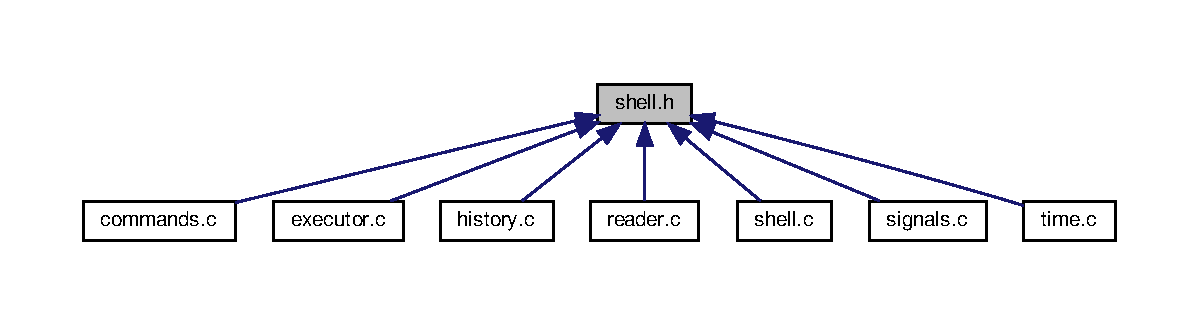
\includegraphics[width=350pt]{shell_8h__dep__incl}
\end{center}
\end{figure}
\subsection*{Macros}
\begin{DoxyCompactItemize}
\item 
\mbox{\Hypertarget{shell_8h_a2f8864f32c9b96956a018e9fedee05db}\label{shell_8h_a2f8864f32c9b96956a018e9fedee05db}} 
\#define \hyperlink{shell_8h_a2f8864f32c9b96956a018e9fedee05db}{H\+I\+S\+T\+O\+R\+Y\+\_\+\+F\+I\+L\+E\+\_\+\+N\+A\+ME}~\char`\"{}/.shellhistory\char`\"{}
\begin{DoxyCompactList}\small\item\em Name of file storing commands history, path is always set to users home directory. \end{DoxyCompactList}\item 
\mbox{\Hypertarget{shell_8h_a88c39f88683d49ba3017df82080ff918}\label{shell_8h_a88c39f88683d49ba3017df82080ff918}} 
\#define \hyperlink{shell_8h_a88c39f88683d49ba3017df82080ff918}{C\+O\+M\+M\+A\+N\+D\+S\+\_\+\+H\+I\+S\+T\+O\+R\+Y\+\_\+\+S\+I\+ZE}~20
\begin{DoxyCompactList}\small\item\em Number of commands to store in commands history file. \end{DoxyCompactList}\item 
\mbox{\Hypertarget{shell_8h_aa9b8dcc02cea15aab8e3d0b7860327a7}\label{shell_8h_aa9b8dcc02cea15aab8e3d0b7860327a7}} 
\#define \hyperlink{shell_8h_aa9b8dcc02cea15aab8e3d0b7860327a7}{I\+N\+P\+U\+T\+\_\+\+B\+U\+F\+F\+E\+R\+\_\+\+S\+I\+ZE}~1024
\begin{DoxyCompactList}\small\item\em Maximum number of characters in single input line. \end{DoxyCompactList}\item 
\mbox{\Hypertarget{shell_8h_a384e42d16491cc03c715918295c450a5}\label{shell_8h_a384e42d16491cc03c715918295c450a5}} 
\#define \hyperlink{shell_8h_a384e42d16491cc03c715918295c450a5}{C\+O\+M\+M\+A\+N\+D\+\_\+\+P\+R\+O\+M\+P\+T\+\_\+\+M\+A\+X\+\_\+\+S\+I\+ZE}~128
\begin{DoxyCompactList}\small\item\em Maximum number of characters in command prompt. \end{DoxyCompactList}\item 
\mbox{\Hypertarget{shell_8h_ac5416897ee25694273cbe9ee32bae0d0}\label{shell_8h_ac5416897ee25694273cbe9ee32bae0d0}} 
\#define \hyperlink{shell_8h_ac5416897ee25694273cbe9ee32bae0d0}{A\+R\+G\+U\+M\+E\+N\+T\+\_\+\+B\+U\+F\+F\+E\+R\+\_\+\+S\+I\+ZE}~64
\begin{DoxyCompactList}\small\item\em Maximum number of parameters for single command. \end{DoxyCompactList}\item 
\mbox{\Hypertarget{shell_8h_ad740dfc826a6f447cf2c273f0fdfe74a}\label{shell_8h_ad740dfc826a6f447cf2c273f0fdfe74a}} 
\#define \hyperlink{shell_8h_ad740dfc826a6f447cf2c273f0fdfe74a}{D\+E\+L\+I\+M\+I\+T\+E\+RS}~\char`\"{} \textbackslash{}t\textbackslash{}r\textbackslash{}n\textbackslash{}a\char`\"{}
\begin{DoxyCompactList}\small\item\em Command arguments delimiters. \end{DoxyCompactList}\end{DoxyCompactItemize}
\subsection*{Functions}
\begin{DoxyCompactItemize}
\item 
int \hyperlink{shell_8h_a069f9558baae3a064ba0e1b54456ccab}{cd} (char $\ast$$\ast$args)
\begin{DoxyCompactList}\small\item\em Change directory command. \end{DoxyCompactList}\item 
void \hyperlink{shell_8h_ada7f892aa09adca3647631590ca1beb0}{clean\+\_\+up} ()
\begin{DoxyCompactList}\small\item\em Cleans up before exit. \end{DoxyCompactList}\item 
int \hyperlink{shell_8h_a3224f605963ffa2708e3e4cc3d8bb41e}{execute\+\_\+command} (int command\+\_\+number, char $\ast$$\ast$args)
\begin{DoxyCompactList}\small\item\em Calls built-\/in command. \end{DoxyCompactList}\item 
int \hyperlink{shell_8h_a38ce9fb8be12b03640a8f1c94a8e4f2c}{execute\+\_\+command\+\_\+or\+\_\+program} (char $\ast$$\ast$args)
\begin{DoxyCompactList}\small\item\em Calls built-\/in command or executes external program. \end{DoxyCompactList}\item 
int \hyperlink{shell_8h_a686fef0ad33bc5f90fcabc31276090f5}{execute\+\_\+program} (char $\ast$$\ast$args, int exec\+\_\+in\+\_\+bg)
\begin{DoxyCompactList}\small\item\em Executes external program. \end{DoxyCompactList}\item 
char $\ast$ \hyperlink{shell_8h_ae312feb7989ddb743fe0b9d2b7995304}{get\+\_\+current\+\_\+time} ()
\begin{DoxyCompactList}\small\item\em Gets system time and converts it to yyyy-\/\+M\+M-\/dd hh\+:mm\+:ss format. \end{DoxyCompactList}\item 
int \hyperlink{shell_8h_a13166be76043b3dfccc0f830c846dc26}{help} ()
\begin{DoxyCompactList}\small\item\em Prints list of built-\/in commands and other functionalities. \end{DoxyCompactList}\item 
\mbox{\Hypertarget{shell_8h_a5fb80f885af4c12056db03cc45a6aae9}\label{shell_8h_a5fb80f885af4c12056db03cc45a6aae9}} 
void \hyperlink{shell_8h_a5fb80f885af4c12056db03cc45a6aae9}{history\+\_\+clean\+\_\+up} ()
\begin{DoxyCompactList}\small\item\em Frees memory, saves commands history to file. \end{DoxyCompactList}\item 
void \hyperlink{shell_8h_ae8516142b2cb36ede692dfca4a36d8cc}{initialize\+\_\+commands\+\_\+history} ()
\begin{DoxyCompactList}\small\item\em Initializes commands history. \end{DoxyCompactList}\item 
\mbox{\Hypertarget{shell_8h_aa2deaf0f63ca4a73a37b86d05678fb46}\label{shell_8h_aa2deaf0f63ca4a73a37b86d05678fb46}} 
void \hyperlink{shell_8h_aa2deaf0f63ca4a73a37b86d05678fb46}{main\+\_\+loop} ()
\begin{DoxyCompactList}\small\item\em Waits for input and executes it. \end{DoxyCompactList}\item 
void \hyperlink{shell_8h_a87a73ece208da0ed13ff48923efa6a8f}{main\+\_\+loop\+\_\+file} (char $\ast$filename)
\begin{DoxyCompactList}\small\item\em Reads script file and executes every line. \end{DoxyCompactList}\item 
int \hyperlink{shell_8h_abcf676d5284d55cb7835a81a80619a48}{print\+\_\+history} ()
\begin{DoxyCompactList}\small\item\em Prints commands history to standard output. \end{DoxyCompactList}\item 
void \hyperlink{shell_8h_a5b063ff4b62fde90e1a44e8c89d5ebc6}{print\+\_\+process\+\_\+signal} (int signum)
\begin{DoxyCompactList}\small\item\em Prints information witch process has been killed. \end{DoxyCompactList}\item 
void \hyperlink{shell_8h_a21579a20737c3b2b24e18bb5e51d8140}{print\+\_\+prompt} ()
\begin{DoxyCompactList}\small\item\em Prints command prompt. \end{DoxyCompactList}\item 
int \hyperlink{shell_8h_a480f710944fe509e060ee055ff64fa88}{print\+\_\+time} ()
\begin{DoxyCompactList}\small\item\em Prints current date and time. \end{DoxyCompactList}\item 
\mbox{\Hypertarget{shell_8h_a6d4d28fe8b4a7cad21ec581450abe1b1}\label{shell_8h_a6d4d28fe8b4a7cad21ec581450abe1b1}} 
void \hyperlink{shell_8h_a6d4d28fe8b4a7cad21ec581450abe1b1}{read\+\_\+clean\+\_\+up} ()
\begin{DoxyCompactList}\small\item\em Frees memory. \end{DoxyCompactList}\item 
char $\ast$ \hyperlink{shell_8h_a777131faf4806e7eee788b65cab4a584}{read\+\_\+line} ()
\begin{DoxyCompactList}\small\item\em Reads one line from standard input. \end{DoxyCompactList}\item 
\mbox{\Hypertarget{shell_8h_ac4ba99969792ae3f877c857cedb129a9}\label{shell_8h_ac4ba99969792ae3f877c857cedb129a9}} 
void \hyperlink{shell_8h_ac4ba99969792ae3f877c857cedb129a9}{save\+\_\+history\+\_\+to\+\_\+file} ()
\begin{DoxyCompactList}\small\item\em Saves command\+\_\+history array to file. \end{DoxyCompactList}\item 
void \hyperlink{shell_8h_aca67f770a00272dc2993db7d854c9c48}{save\+\_\+to\+\_\+history} (char $\ast$input)
\begin{DoxyCompactList}\small\item\em Saves command to history. \end{DoxyCompactList}\item 
void \hyperlink{shell_8h_a6af3c0bed2d48bb950788acf54f4de74}{signals\+\_\+handler} (int signum)
\begin{DoxyCompactList}\small\item\em Handles signals. \end{DoxyCompactList}\item 
char $\ast$$\ast$ \hyperlink{shell_8h_a9c985d892b630e70b2236554b46faa4b}{split\+\_\+input} (char $\ast$input)
\begin{DoxyCompactList}\small\item\em Splits input to words (command and its arguments). \end{DoxyCompactList}\item 
\mbox{\Hypertarget{shell_8h_a62b3e552188dc2021715c1be2bd60267}\label{shell_8h_a62b3e552188dc2021715c1be2bd60267}} 
void \hyperlink{shell_8h_a62b3e552188dc2021715c1be2bd60267}{update\+\_\+prompt} ()
\begin{DoxyCompactList}\small\item\em Updates prompt with username and current path. \end{DoxyCompactList}\end{DoxyCompactItemize}


\subsection{Detailed Description}
\begin{DoxyAuthor}{Author}
Mateusz Wawreszuk 
\end{DoxyAuthor}


\subsection{Function Documentation}
\mbox{\Hypertarget{shell_8h_a069f9558baae3a064ba0e1b54456ccab}\label{shell_8h_a069f9558baae3a064ba0e1b54456ccab}} 
\index{shell.\+h@{shell.\+h}!cd@{cd}}
\index{cd@{cd}!shell.\+h@{shell.\+h}}
\subsubsection{\texorpdfstring{cd()}{cd()}}
{\footnotesize\ttfamily int cd (\begin{DoxyParamCaption}\item[{char $\ast$$\ast$}]{args }\end{DoxyParamCaption})}



Change directory command. 

If change is not possible, prints to standard output error message.


\begin{DoxyParams}{Parameters}
{\em args} & directory \\
\hline
\end{DoxyParams}
\begin{DoxyReturn}{Returns}
execution success or error code 
\end{DoxyReturn}
\mbox{\Hypertarget{shell_8h_ada7f892aa09adca3647631590ca1beb0}\label{shell_8h_ada7f892aa09adca3647631590ca1beb0}} 
\index{shell.\+h@{shell.\+h}!clean\+\_\+up@{clean\+\_\+up}}
\index{clean\+\_\+up@{clean\+\_\+up}!shell.\+h@{shell.\+h}}
\subsubsection{\texorpdfstring{clean\+\_\+up()}{clean\_up()}}
{\footnotesize\ttfamily void clean\+\_\+up (\begin{DoxyParamCaption}{ }\end{DoxyParamCaption})}



Cleans up before exit. 

Frees memory and saves commands history to file. \mbox{\Hypertarget{shell_8h_a3224f605963ffa2708e3e4cc3d8bb41e}\label{shell_8h_a3224f605963ffa2708e3e4cc3d8bb41e}} 
\index{shell.\+h@{shell.\+h}!execute\+\_\+command@{execute\+\_\+command}}
\index{execute\+\_\+command@{execute\+\_\+command}!shell.\+h@{shell.\+h}}
\subsubsection{\texorpdfstring{execute\+\_\+command()}{execute\_command()}}
{\footnotesize\ttfamily int execute\+\_\+command (\begin{DoxyParamCaption}\item[{int}]{command\+\_\+number,  }\item[{char $\ast$$\ast$}]{args }\end{DoxyParamCaption})}



Calls built-\/in command. 


\begin{DoxyParams}{Parameters}
{\em command\+\_\+number} & number of command in built\+\_\+in\+\_\+commands array \\
\hline
{\em args} & arguments \\
\hline
\end{DoxyParams}
\begin{DoxyReturn}{Returns}
execution success or error code 
\end{DoxyReturn}
\mbox{\Hypertarget{shell_8h_a38ce9fb8be12b03640a8f1c94a8e4f2c}\label{shell_8h_a38ce9fb8be12b03640a8f1c94a8e4f2c}} 
\index{shell.\+h@{shell.\+h}!execute\+\_\+command\+\_\+or\+\_\+program@{execute\+\_\+command\+\_\+or\+\_\+program}}
\index{execute\+\_\+command\+\_\+or\+\_\+program@{execute\+\_\+command\+\_\+or\+\_\+program}!shell.\+h@{shell.\+h}}
\subsubsection{\texorpdfstring{execute\+\_\+command\+\_\+or\+\_\+program()}{execute\_command\_or\_program()}}
{\footnotesize\ttfamily int execute\+\_\+command\+\_\+or\+\_\+program (\begin{DoxyParamCaption}\item[{char $\ast$$\ast$}]{args }\end{DoxyParamCaption})}



Calls built-\/in command or executes external program. 

Checks if program should be executed in background (first argument is \char`\"{}\&\char`\"{}).


\begin{DoxyParams}{Parameters}
{\em args} & array of command and its arguments \\
\hline
\end{DoxyParams}
\begin{DoxyReturn}{Returns}
execution success or error code 
\end{DoxyReturn}
\mbox{\Hypertarget{shell_8h_a686fef0ad33bc5f90fcabc31276090f5}\label{shell_8h_a686fef0ad33bc5f90fcabc31276090f5}} 
\index{shell.\+h@{shell.\+h}!execute\+\_\+program@{execute\+\_\+program}}
\index{execute\+\_\+program@{execute\+\_\+program}!shell.\+h@{shell.\+h}}
\subsubsection{\texorpdfstring{execute\+\_\+program()}{execute\_program()}}
{\footnotesize\ttfamily int execute\+\_\+program (\begin{DoxyParamCaption}\item[{char $\ast$$\ast$}]{args,  }\item[{int}]{exec\+\_\+in\+\_\+bg }\end{DoxyParamCaption})}



Executes external program. 


\begin{DoxyParams}{Parameters}
{\em args} & array of command and its arguments \\
\hline
{\em exec\+\_\+in\+\_\+bg} & 1 if program should be executed in background, 0 if not \\
\hline
\end{DoxyParams}
\begin{DoxyReturn}{Returns}
W\+Y\+J\+S\+C\+IE 
\end{DoxyReturn}
\mbox{\Hypertarget{shell_8h_ae312feb7989ddb743fe0b9d2b7995304}\label{shell_8h_ae312feb7989ddb743fe0b9d2b7995304}} 
\index{shell.\+h@{shell.\+h}!get\+\_\+current\+\_\+time@{get\+\_\+current\+\_\+time}}
\index{get\+\_\+current\+\_\+time@{get\+\_\+current\+\_\+time}!shell.\+h@{shell.\+h}}
\subsubsection{\texorpdfstring{get\+\_\+current\+\_\+time()}{get\_current\_time()}}
{\footnotesize\ttfamily char$\ast$ get\+\_\+current\+\_\+time (\begin{DoxyParamCaption}{ }\end{DoxyParamCaption})}



Gets system time and converts it to yyyy-\/\+M\+M-\/dd hh\+:mm\+:ss format. 

\begin{DoxyReturn}{Returns}
current local time as char array 
\end{DoxyReturn}
\mbox{\Hypertarget{shell_8h_a13166be76043b3dfccc0f830c846dc26}\label{shell_8h_a13166be76043b3dfccc0f830c846dc26}} 
\index{shell.\+h@{shell.\+h}!help@{help}}
\index{help@{help}!shell.\+h@{shell.\+h}}
\subsubsection{\texorpdfstring{help()}{help()}}
{\footnotesize\ttfamily int help (\begin{DoxyParamCaption}{ }\end{DoxyParamCaption})}



Prints list of built-\/in commands and other functionalities. 

\begin{DoxyReturn}{Returns}
success code 
\end{DoxyReturn}
\mbox{\Hypertarget{shell_8h_ae8516142b2cb36ede692dfca4a36d8cc}\label{shell_8h_ae8516142b2cb36ede692dfca4a36d8cc}} 
\index{shell.\+h@{shell.\+h}!initialize\+\_\+commands\+\_\+history@{initialize\+\_\+commands\+\_\+history}}
\index{initialize\+\_\+commands\+\_\+history@{initialize\+\_\+commands\+\_\+history}!shell.\+h@{shell.\+h}}
\subsubsection{\texorpdfstring{initialize\+\_\+commands\+\_\+history()}{initialize\_commands\_history()}}
{\footnotesize\ttfamily void initialize\+\_\+commands\+\_\+history (\begin{DoxyParamCaption}{ }\end{DoxyParamCaption})}



Initializes commands history. 

Allocates commands\+\_\+history array and reads current history from file. Sets history\+\_\+counter pointer to commands\+\_\+history size. \mbox{\Hypertarget{shell_8h_a87a73ece208da0ed13ff48923efa6a8f}\label{shell_8h_a87a73ece208da0ed13ff48923efa6a8f}} 
\index{shell.\+h@{shell.\+h}!main\+\_\+loop\+\_\+file@{main\+\_\+loop\+\_\+file}}
\index{main\+\_\+loop\+\_\+file@{main\+\_\+loop\+\_\+file}!shell.\+h@{shell.\+h}}
\subsubsection{\texorpdfstring{main\+\_\+loop\+\_\+file()}{main\_loop\_file()}}
{\footnotesize\ttfamily void main\+\_\+loop\+\_\+file (\begin{DoxyParamCaption}\item[{char $\ast$}]{filename }\end{DoxyParamCaption})}



Reads script file and executes every line. 


\begin{DoxyParams}{Parameters}
{\em filename} & script file name and path \\
\hline
\end{DoxyParams}
\mbox{\Hypertarget{shell_8h_abcf676d5284d55cb7835a81a80619a48}\label{shell_8h_abcf676d5284d55cb7835a81a80619a48}} 
\index{shell.\+h@{shell.\+h}!print\+\_\+history@{print\+\_\+history}}
\index{print\+\_\+history@{print\+\_\+history}!shell.\+h@{shell.\+h}}
\subsubsection{\texorpdfstring{print\+\_\+history()}{print\_history()}}
{\footnotesize\ttfamily int print\+\_\+history (\begin{DoxyParamCaption}{ }\end{DoxyParamCaption})}



Prints commands history to standard output. 

\begin{DoxyReturn}{Returns}
success code 
\end{DoxyReturn}
\mbox{\Hypertarget{shell_8h_a5b063ff4b62fde90e1a44e8c89d5ebc6}\label{shell_8h_a5b063ff4b62fde90e1a44e8c89d5ebc6}} 
\index{shell.\+h@{shell.\+h}!print\+\_\+process\+\_\+signal@{print\+\_\+process\+\_\+signal}}
\index{print\+\_\+process\+\_\+signal@{print\+\_\+process\+\_\+signal}!shell.\+h@{shell.\+h}}
\subsubsection{\texorpdfstring{print\+\_\+process\+\_\+signal()}{print\_process\_signal()}}
{\footnotesize\ttfamily void print\+\_\+process\+\_\+signal (\begin{DoxyParamCaption}\item[{int}]{signum }\end{DoxyParamCaption})}



Prints information witch process has been killed. 


\begin{DoxyParams}{Parameters}
{\em signum} & signal number \\
\hline
\end{DoxyParams}
\mbox{\Hypertarget{shell_8h_a21579a20737c3b2b24e18bb5e51d8140}\label{shell_8h_a21579a20737c3b2b24e18bb5e51d8140}} 
\index{shell.\+h@{shell.\+h}!print\+\_\+prompt@{print\+\_\+prompt}}
\index{print\+\_\+prompt@{print\+\_\+prompt}!shell.\+h@{shell.\+h}}
\subsubsection{\texorpdfstring{print\+\_\+prompt()}{print\_prompt()}}
{\footnotesize\ttfamily void print\+\_\+prompt (\begin{DoxyParamCaption}{ }\end{DoxyParamCaption})}



Prints command prompt. 

Command prompt contains\+: current user, current working directory, \# if current user is superuser or \$ for other users \mbox{\Hypertarget{shell_8h_a480f710944fe509e060ee055ff64fa88}\label{shell_8h_a480f710944fe509e060ee055ff64fa88}} 
\index{shell.\+h@{shell.\+h}!print\+\_\+time@{print\+\_\+time}}
\index{print\+\_\+time@{print\+\_\+time}!shell.\+h@{shell.\+h}}
\subsubsection{\texorpdfstring{print\+\_\+time()}{print\_time()}}
{\footnotesize\ttfamily int print\+\_\+time (\begin{DoxyParamCaption}{ }\end{DoxyParamCaption})}



Prints current date and time. 

\begin{DoxyReturn}{Returns}
success code 
\end{DoxyReturn}
\mbox{\Hypertarget{shell_8h_a777131faf4806e7eee788b65cab4a584}\label{shell_8h_a777131faf4806e7eee788b65cab4a584}} 
\index{shell.\+h@{shell.\+h}!read\+\_\+line@{read\+\_\+line}}
\index{read\+\_\+line@{read\+\_\+line}!shell.\+h@{shell.\+h}}
\subsubsection{\texorpdfstring{read\+\_\+line()}{read\_line()}}
{\footnotesize\ttfamily char$\ast$ read\+\_\+line (\begin{DoxyParamCaption}{ }\end{DoxyParamCaption})}



Reads one line from standard input. 

\begin{DoxyReturn}{Returns}
line as char array 
\end{DoxyReturn}
\mbox{\Hypertarget{shell_8h_aca67f770a00272dc2993db7d854c9c48}\label{shell_8h_aca67f770a00272dc2993db7d854c9c48}} 
\index{shell.\+h@{shell.\+h}!save\+\_\+to\+\_\+history@{save\+\_\+to\+\_\+history}}
\index{save\+\_\+to\+\_\+history@{save\+\_\+to\+\_\+history}!shell.\+h@{shell.\+h}}
\subsubsection{\texorpdfstring{save\+\_\+to\+\_\+history()}{save\_to\_history()}}
{\footnotesize\ttfamily void save\+\_\+to\+\_\+history (\begin{DoxyParamCaption}\item[{char $\ast$}]{input }\end{DoxyParamCaption})}



Saves command to history. 

If history\+\_\+counter pointer points that history is full, removes first command from history.


\begin{DoxyParams}{Parameters}
{\em input} & command to save \\
\hline
\end{DoxyParams}
\mbox{\Hypertarget{shell_8h_a6af3c0bed2d48bb950788acf54f4de74}\label{shell_8h_a6af3c0bed2d48bb950788acf54f4de74}} 
\index{shell.\+h@{shell.\+h}!signals\+\_\+handler@{signals\+\_\+handler}}
\index{signals\+\_\+handler@{signals\+\_\+handler}!shell.\+h@{shell.\+h}}
\subsubsection{\texorpdfstring{signals\+\_\+handler()}{signals\_handler()}}
{\footnotesize\ttfamily void signals\+\_\+handler (\begin{DoxyParamCaption}\item[{int}]{signum }\end{DoxyParamCaption})}



Handles signals. 

Handled signals\+: S\+I\+G\+Q\+U\+IT, S\+I\+G\+I\+NT, S\+I\+G\+T\+S\+TP.


\begin{DoxyParams}{Parameters}
{\em signum} & signal number \\
\hline
\end{DoxyParams}
\mbox{\Hypertarget{shell_8h_a9c985d892b630e70b2236554b46faa4b}\label{shell_8h_a9c985d892b630e70b2236554b46faa4b}} 
\index{shell.\+h@{shell.\+h}!split\+\_\+input@{split\+\_\+input}}
\index{split\+\_\+input@{split\+\_\+input}!shell.\+h@{shell.\+h}}
\subsubsection{\texorpdfstring{split\+\_\+input()}{split\_input()}}
{\footnotesize\ttfamily char$\ast$$\ast$ split\+\_\+input (\begin{DoxyParamCaption}\item[{char $\ast$}]{input }\end{DoxyParamCaption})}



Splits input to words (command and its arguments). 


\begin{DoxyParams}{Parameters}
{\em input} & single input line \\
\hline
\end{DoxyParams}
\begin{DoxyReturn}{Returns}
array of command and arguments 
\end{DoxyReturn}

\hypertarget{signals_8c}{}\section{signals.\+c File Reference}
\label{signals_8c}\index{signals.\+c@{signals.\+c}}
{\ttfamily \#include \char`\"{}shell.\+h\char`\"{}}\newline
\subsection*{Functions}
\begin{DoxyCompactItemize}
\item 
void \hyperlink{signals_8c_a6af3c0bed2d48bb950788acf54f4de74}{signals\+\_\+handler} (int signum)
\begin{DoxyCompactList}\small\item\em Handles signals. \end{DoxyCompactList}\end{DoxyCompactItemize}


\subsection{Detailed Description}
\begin{DoxyAuthor}{Author}
Mateusz Wawreszuk 
\end{DoxyAuthor}


\subsection{Function Documentation}
\mbox{\Hypertarget{signals_8c_a6af3c0bed2d48bb950788acf54f4de74}\label{signals_8c_a6af3c0bed2d48bb950788acf54f4de74}} 
\index{signals.\+c@{signals.\+c}!signals\+\_\+handler@{signals\+\_\+handler}}
\index{signals\+\_\+handler@{signals\+\_\+handler}!signals.\+c@{signals.\+c}}
\subsubsection{\texorpdfstring{signals\+\_\+handler()}{signals\_handler()}}
{\footnotesize\ttfamily void signals\+\_\+handler (\begin{DoxyParamCaption}\item[{int}]{signum }\end{DoxyParamCaption})}



Handles signals. 

Handled signals\+: S\+I\+G\+Q\+U\+IT, S\+I\+G\+I\+NT, S\+I\+G\+T\+S\+TP.


\begin{DoxyParams}{Parameters}
{\em signum} & signal number \\
\hline
\end{DoxyParams}

\hypertarget{time_8c}{}\section{time.\+c File Reference}
\label{time_8c}\index{time.\+c@{time.\+c}}
{\ttfamily \#include \char`\"{}shell.\+h\char`\"{}}\newline
\subsection*{Functions}
\begin{DoxyCompactItemize}
\item 
char $\ast$ \hyperlink{time_8c_ae312feb7989ddb743fe0b9d2b7995304}{get\+\_\+current\+\_\+time} ()
\begin{DoxyCompactList}\small\item\em Gets system time and converts it to yyyy-\/\+M\+M-\/dd hh\+:mm\+:ss format. \end{DoxyCompactList}\end{DoxyCompactItemize}


\subsection{Detailed Description}
\begin{DoxyAuthor}{Author}
Mateusz Wawreszuk 
\end{DoxyAuthor}


\subsection{Function Documentation}
\mbox{\Hypertarget{time_8c_ae312feb7989ddb743fe0b9d2b7995304}\label{time_8c_ae312feb7989ddb743fe0b9d2b7995304}} 
\index{time.\+c@{time.\+c}!get\+\_\+current\+\_\+time@{get\+\_\+current\+\_\+time}}
\index{get\+\_\+current\+\_\+time@{get\+\_\+current\+\_\+time}!time.\+c@{time.\+c}}
\subsubsection{\texorpdfstring{get\+\_\+current\+\_\+time()}{get\_current\_time()}}
{\footnotesize\ttfamily char$\ast$ get\+\_\+current\+\_\+time (\begin{DoxyParamCaption}{ }\end{DoxyParamCaption})}



Gets system time and converts it to yyyy-\/\+M\+M-\/dd hh\+:mm\+:ss format. 

\begin{DoxyReturn}{Returns}
current local time as char array 
\end{DoxyReturn}

%--- End generated contents ---

% Index
\backmatter
\newpage
\phantomsection
\clearemptydoublepage
\addcontentsline{toc}{chapter}{Index}
\printindex

\end{document}
